\documentclass{styles/svproc}
\usepackage{url}
\usepackage{makeidx}
\usepackage[utf8]{inputenc}
\usepackage{graphicx}
\graphicspath{ {img/} }

\begin{document}

\title{Fine 3D path following of a quadcopter}
\author{Manuel Zafra Villar\inst{1} \and Jose María Cañas Plaza\inst{2}}
\institute{Universidad Rey Juan Carlos, Madrid, Spain}
\titlerunning{Fine 3D path following of a quadcopter}
\maketitle

\begin{abstract}
This paper addresses the design and implementation of a path following controlling system for a drone which relies on 3D localization by visual markers. It has been designed only for indoor flights. Special attention is paid to accuracy of the position estimation algorithm, robustness of the path following controller and real time operation. The path following system is composed of two components, one responsible of the image analysis and 3D pose estimation and another responsible of the drone navigation. It has been experimentally validated both in Gazebo simulator and in a real drone. 
\end{abstract}

\section{Introduction}

	In recent years, 
%the rapid development of new technologies and the decreasing price of the hardware have allowed an easier access to robotics. There has also
there has been an emerging interest in the use of \textit{Unmaned Aerial Vehicles} (UAVs) with applications such as 3D mapping, military tasks, security, inspection \cite{nikolic2014} or agriculture. Maybe quadrotors are the most popular aerial vehicles now. Currently there are several lines of research and projects with UAVs, including prototypes from big companies like \textit{Project Wing} from \textit{Google} or \textit{Prime Air} from \textit{Amazon}. 
 %competitions
        This growing interest in aerial robotics also is reflected in several international competitions like Int. Micro Air Vehicle Indoor Flight Competition IMAV \footnote{http://www.imavs.org}, DronesForGood \footnote{http://www.dronesforgood.ae}, Mohamed Bin Zayed Int. Robotics Challenge (MBZIRC) \footnote{http://www.mbzirc.com}, which foster the research and development of UAVs technology.


        %frameworks
	In order to accomplish some of the above mentioned taks, the aerial vehicles must work autonomously without the constant supervision of human operators. Many capabilities are desired in this context, like path following, self-localization, precision landing, obstacle detection and avoidance among others. There are several frameworks for UAVs that help in developing such capabilities and provides support for different hardware platforms. For instance, AEROSTACK \cite{sanchezlopez2016}, PX4 Flight Stack \footnote{http://px4.io}, APM Flight Stack \footnote{http://ardupilot.com}, Telekyb \cite{grabe2013}, Hector quadrotor framework \cite{kohlbrecher2014}, beyond other general robotics middlewares like ROS.

        
        % path following
        One important capability to achieve the UAV autonomy is following of predefined paths in 3D \cite{dandrea2015,beul2015,nguyen2014}. For this behavior the UAV should continuously know its 3D position and control its movements to advance through the desired 3D path.

        % self-localization
        3D localization can be achieved in outdoor scenarios with the help of sensors such as GPS, Inertial Measurement Unit (IMU) or altimeter. In indoor environments higher accuracy is needed as there may be multiple obstacles within a few meters. There, solutions may come from external motion capture systems \cite{jimenez2014,lupashin2014,michael2010} or from onboard computer vision \cite{wu2013,rodriguezramos2016}, optionally using IMUs too. Typically motion capture systems monitor the position of the vehicles at a high frequency, like 100 Hz. The procedures may vary depending on the camera used (RGB, RGBD, ToF...) and whether the camera is on the scenario or onboard the drone. When using on board cameras, three main techniques can be distinguished. First, \textit{Visual Odometry} in which the position is estimated by calculating the incremental movement between separate pictures extracting feature points of images. Even though this method can provide good short-term accuracy, the error rapidly increases with movement. Second, \textit{Visual SLAM} family of algorithms allows the mapping of the area observed and simultaneously the localization of the camera. MonoSLAM, PTAM, DSO \cite{engel2017}, LSD-SLAM and SVO \cite{forster2014} algorithms belong to this family. And third, \textit{Localization based on Markers} (fiducial systems), which is based on the previous knowledge of the environment's map \cite{apvrille2013}. The map is a colletion of visual markers whose absolute position is known, so when the camera detects any of them the absolute camera position can be obtained estimatind the relative position camera-marker.
%The markers that can be used are plenty, with the only limitation being that the camera must be able to recognize them easily. Some of the most common markers used are bi-dimensional bar codes, which are the ones used by this system.
	
        % control approaches
        The control of the movements can be achieved with several approaches like PID controllers, fuzzy controllers, Internal Model Control \cite{hernandez2013}, Model Predictive Control (MPC) \cite{hernandez2014}, direct vision-based control \cite{nguyen2014}, etc.. Direct vision-based control has been used in other capabilities like precision landing too.
        
        %% hardware: drones
        %% In this case, we are using a specific UAV type, quadcopters. A quadcopter is a multirotor helicopter that is propelled by four rotors. This kind of aerial vehicle differs from conventional helicopters, which use rotors that are able to vary the pitch of their blades dynamically as they move around the rotor hub. Usually, the architecture consist of two rotors on the front and two on the back, however some models include one frontal rotor, two on the sides and another one on the back. The rotors, when functioning, apply an upwards force called lift that sustain the vehicle. In order to the quadcopter to take off, the lift must be higher than gravitational forces. Once hovering, if gravitational forces equal lift, the vehicle will remaing still. Modifying lift will cause it to go upwards or downwards depending on the force applied. Horizontal movement is generated by altering the rotation power of two pairs of rotors. For instance, if we want to apply forward movement we have to reduce the power of the two frontal rotors and increase power on both of the rear rotors. The difference of the power applied is proportional to the movement speed generated. To understand rotation movement, we have to comprehend how the rotors work in sense of rotational direction. In order to the quadcopter to mantain its position, angular velocity must equal zero. This is accomplished by having two rotors function with one rotational direction and making the opposite pair rotate on the reverse direction. If different power is applied to pairs of rotors, the quadrotor will rotate towards the direction of the most powerful rotors.
	
	The goal of this project is to develop the first prototype of a vision-based path following system for quadcopters in indoor environments. The navigation will be based on a path tracking method, ensuring a robust position control. In order to accomplish that, the self location will depend on computer vision algorithms relying on visual markers. Given the features of the environment, the system should function with minimal spatial errors in order to avoid obstacles in narrow scenarios.

\section{Infrastructure}

Several hardware and software pieces have been used in this work.

\subsection{ArDrone2 quadrotor}

	The hardware platform used is \textit{ArDrone2.0} from Parrot (Figure \ref{fig:calibration}, left). This quadcopter was developed in 2012 as an enhancement over \textit{ArDrone1.0} and its main features are summarized in Table \ref{table:quadrotor}. The onboard computer runs a \textit{Linux} OS, and communicates with the pilot through a self-generated Wi-Fi spot. The onboard sensors include an ultrasonic altimeter enhanced with an air pressure sensor, as well as 3-axis gyroscope, accelerometer and magnetometer, which are used to provide stabilisation. It is also equipped with a 720p front camera and a ventral QVGA sensor.
	
	\begin{table}
	\centering
	\setlength\tabcolsep{7pt}
	\caption{ArDrone2.0 features}
	\begin{tabular}{llllll}
	\hline\noalign{\smallskip}
	Characteristic  & Value\\
	\noalign{\smallskip}
	\hline
	\noalign{\smallskip}
		Size & 58.4 x 1.3 x 58.4 cm. \\
		Weight & 436 g. \\
		Wi-fi range & 50 m. \\
		Max. speed & 18 km/h \\
		Camera  & 1280 x 720 pixels \\
		Max. height & 100 m.\\
	\hline
	\end{tabular}
        \label{table:quadrotor}
	\end{table}

\subsection{AprilTags beacons}

	\textit{AprilTags} is a visual fiducial system widely used for tasks including robotics, augmented reality and camera calibration. This system was developed in 2011 by Ed Olson \cite{eolson}. It is similar to QR Codes, both are two-dimensional bar codes (Fig. \ref{fig:apriltags}), but AprilTags were designed to encode far smaller data payloads (between 4 and 12 bits) and introduces a new encoding system which addresses some specific problems with 2D bar codes. It enhances robust detection in more rotation angles and robustness against false positives, allowing them to be detected from longer ranges.
	
	AprilTags library detects any of its markers in a given image, providing the unique ID of the tag as well as its location (height and width pixel) in the image. It can also provide the relative transformation between tag and camera. For this system, AprilTags has only been used for the detection of tags in the image. The provided position estimation was not used here because we wanted to rely only in our existing 3D self-localization component \cite{lopezceron2016}, which has been also employed in other projects and includes several mechanisms to increase robustness and accuracy.
	
	\begin{figure}[h]
		\begin{center}
		{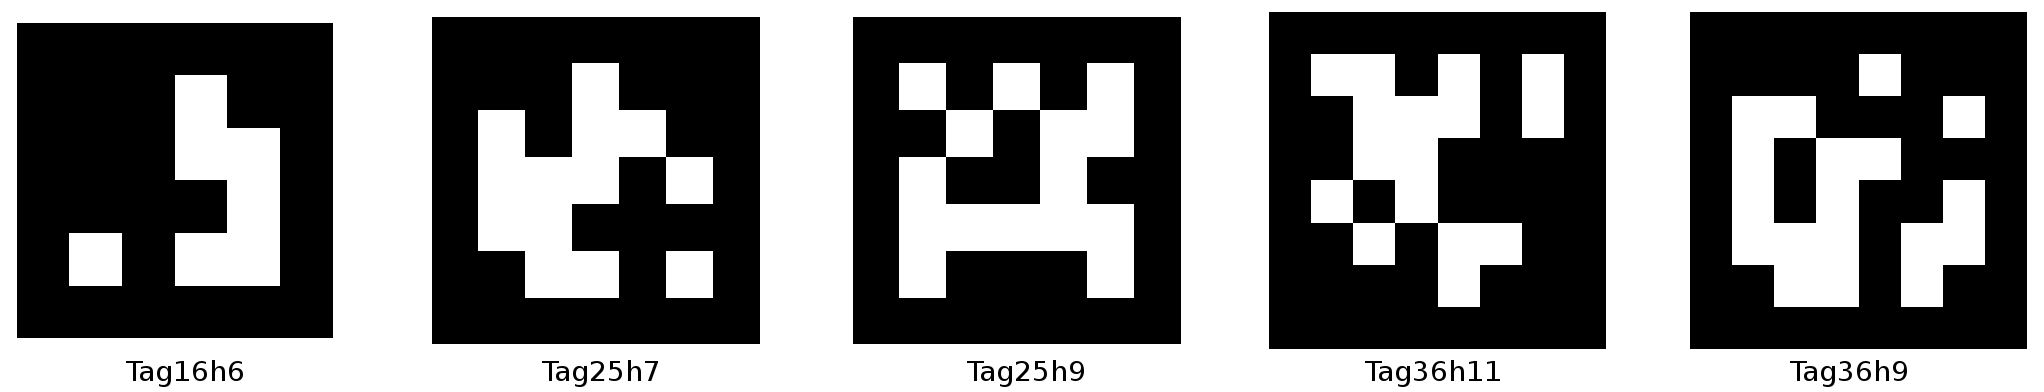
\includegraphics[width=\linewidth]{ejemplosapriltags.png}}
		\end{center}
		\caption{Some examples of AprilTags markers}
		\label{fig:apriltags}
	\end{figure}
	
\subsection{JdeRobot framework}

	The system has been developed using JdeRobot\footnote{http://jderobot.org}, an open source robotics and computer vision development framework.  In this framework robot applications are built from several distributed nodes which communicates themselves trough ICE (\textit{Internet Comunication Engine} from ZeroC) or ROS messages grouped on explicit \textit{interfaces/topics}. It is fully ROS compatible, provides support to many sensors and actuators, several libraries and tools. Some of them are oriented to aerial vehicles. It simplifies hardware access from applications providing an abstraction layer over the manufacturer's software such as \textit{Ar.Drone SDK} in \textit{ArDrone}.

%It is mainly developed in C++, also having some parts developed in Python. In JdeRobot a robotic application typically is composed of several interacting components and the communication between them is done through \textit{Internet Comunication Engine} (ICE) over TCP/IP. ICE is a server-client protocol, based on \textit{Remote Procedure Call} (RPC), which allows remote execution of software without worrying about communications.
% The components may extract information from different robot sensors and provide it for other components. Within JdeRobot there are many drivers developed to support several physical sensors and actuators. 

%        \subsubsection{Progeo Library}
%        JdeRobot also contains several libraries such as \textit{progeo}, \textit{jderobotutil} or \textit{geometry}.
 \textit{Progeo} is a JdeRobot library for projective geometry which offers functions that relate 2D and 3D points. Having the camera extrinsic and intrinsic parameters, obtained by calibration, there is a \textit{project} function that computes the 2D pixel on which a given 3D point in space projects in the image. There is also a \textit{backproject} function that computes the 3D ray containing all the 3D points which projects into the same pixel. 

%        \subsubsection{CameraCalibrator}
 \textit{CameraCalibrator} is a JdeRobot opencv-based tool which obtains the intrinsic parameters of a camera using an intuitive GUI and a calibration pattern. It provides a simple process and a configuration file where settings like calibration pattern, method, number of images taken or delay between images can be changed. It deliver the parameters on a \textit{.yml} output text file.
 %CameraCalibrator recieves camera images by ICE interface, and offers a simple user interface which simplifies the calibration process. 
%In its configuration file, settings can be modified such as calibration pattern, number of images taken or delay between images. The component uses OpenCV and its camera calibration methods and writes the output in a \textit{.yml} text file. 
This tool was used to obtain the camera parameters for the real ArDrone camera (Figure \ref{fig:calibration}, right) and the simulated one.

	\begin{figure}[h]
		\begin{center}
                  {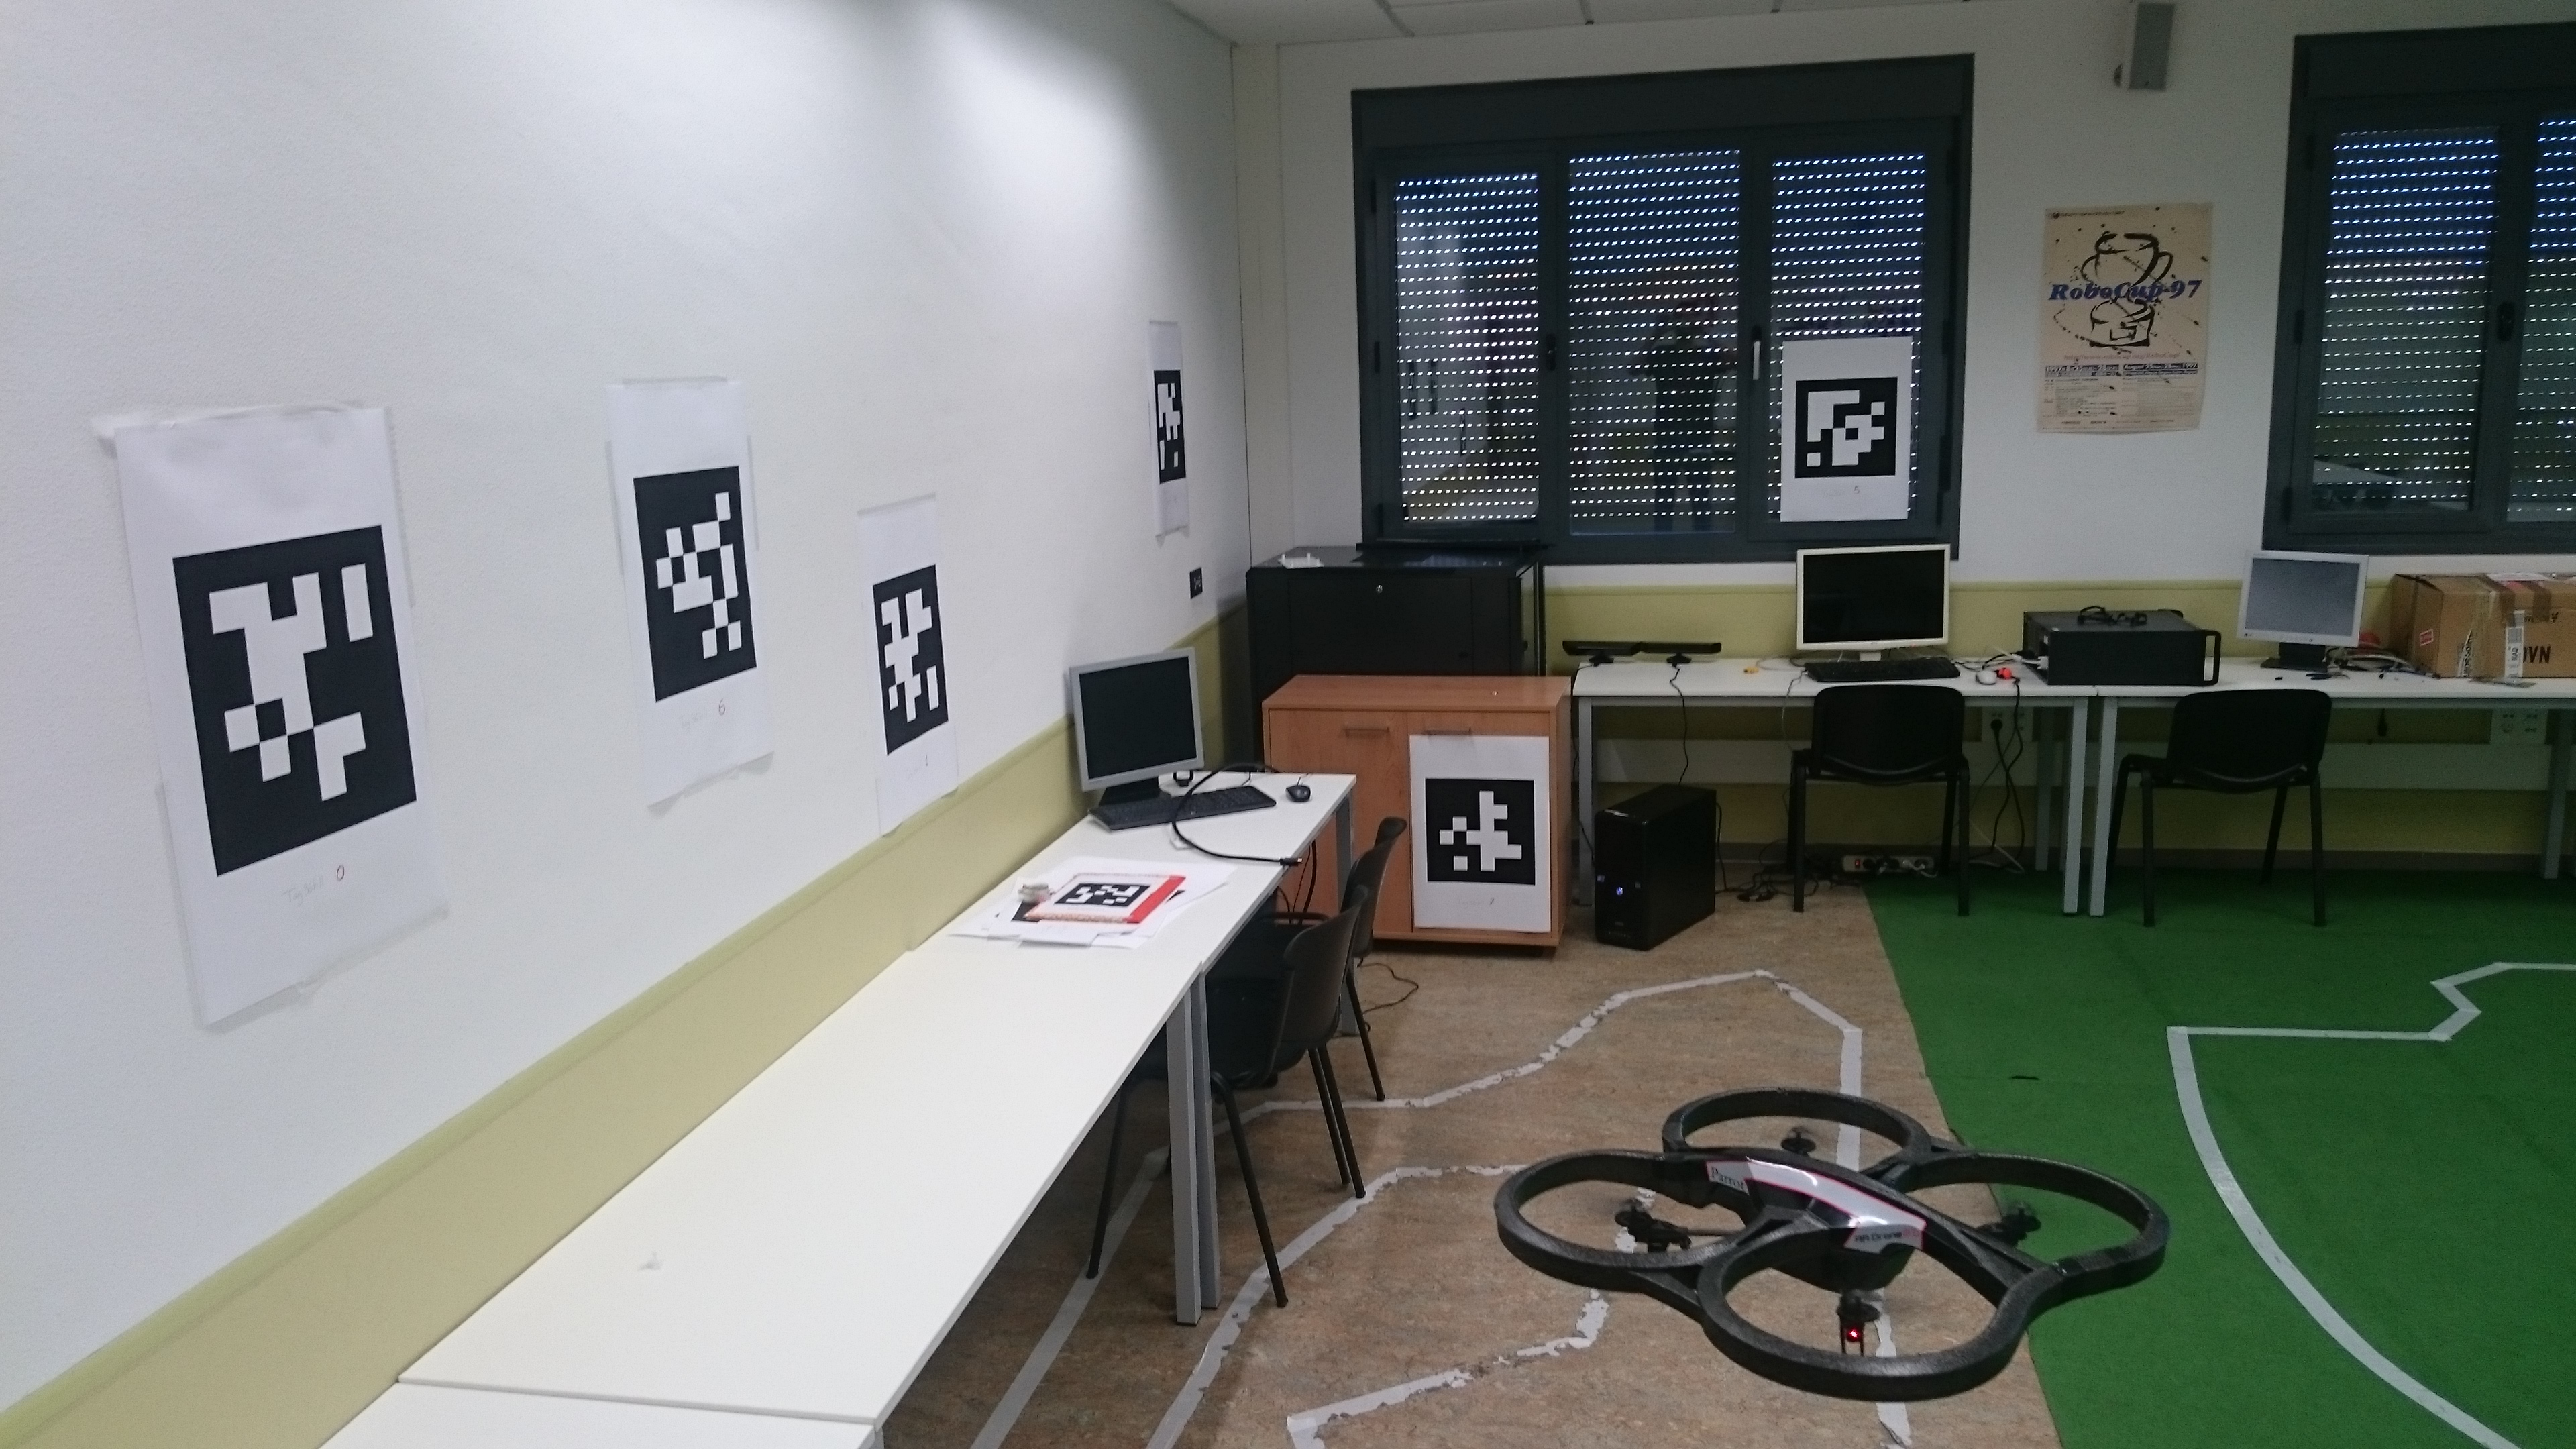
\includegraphics[width=6cm]{realnavigation.png}}
                  {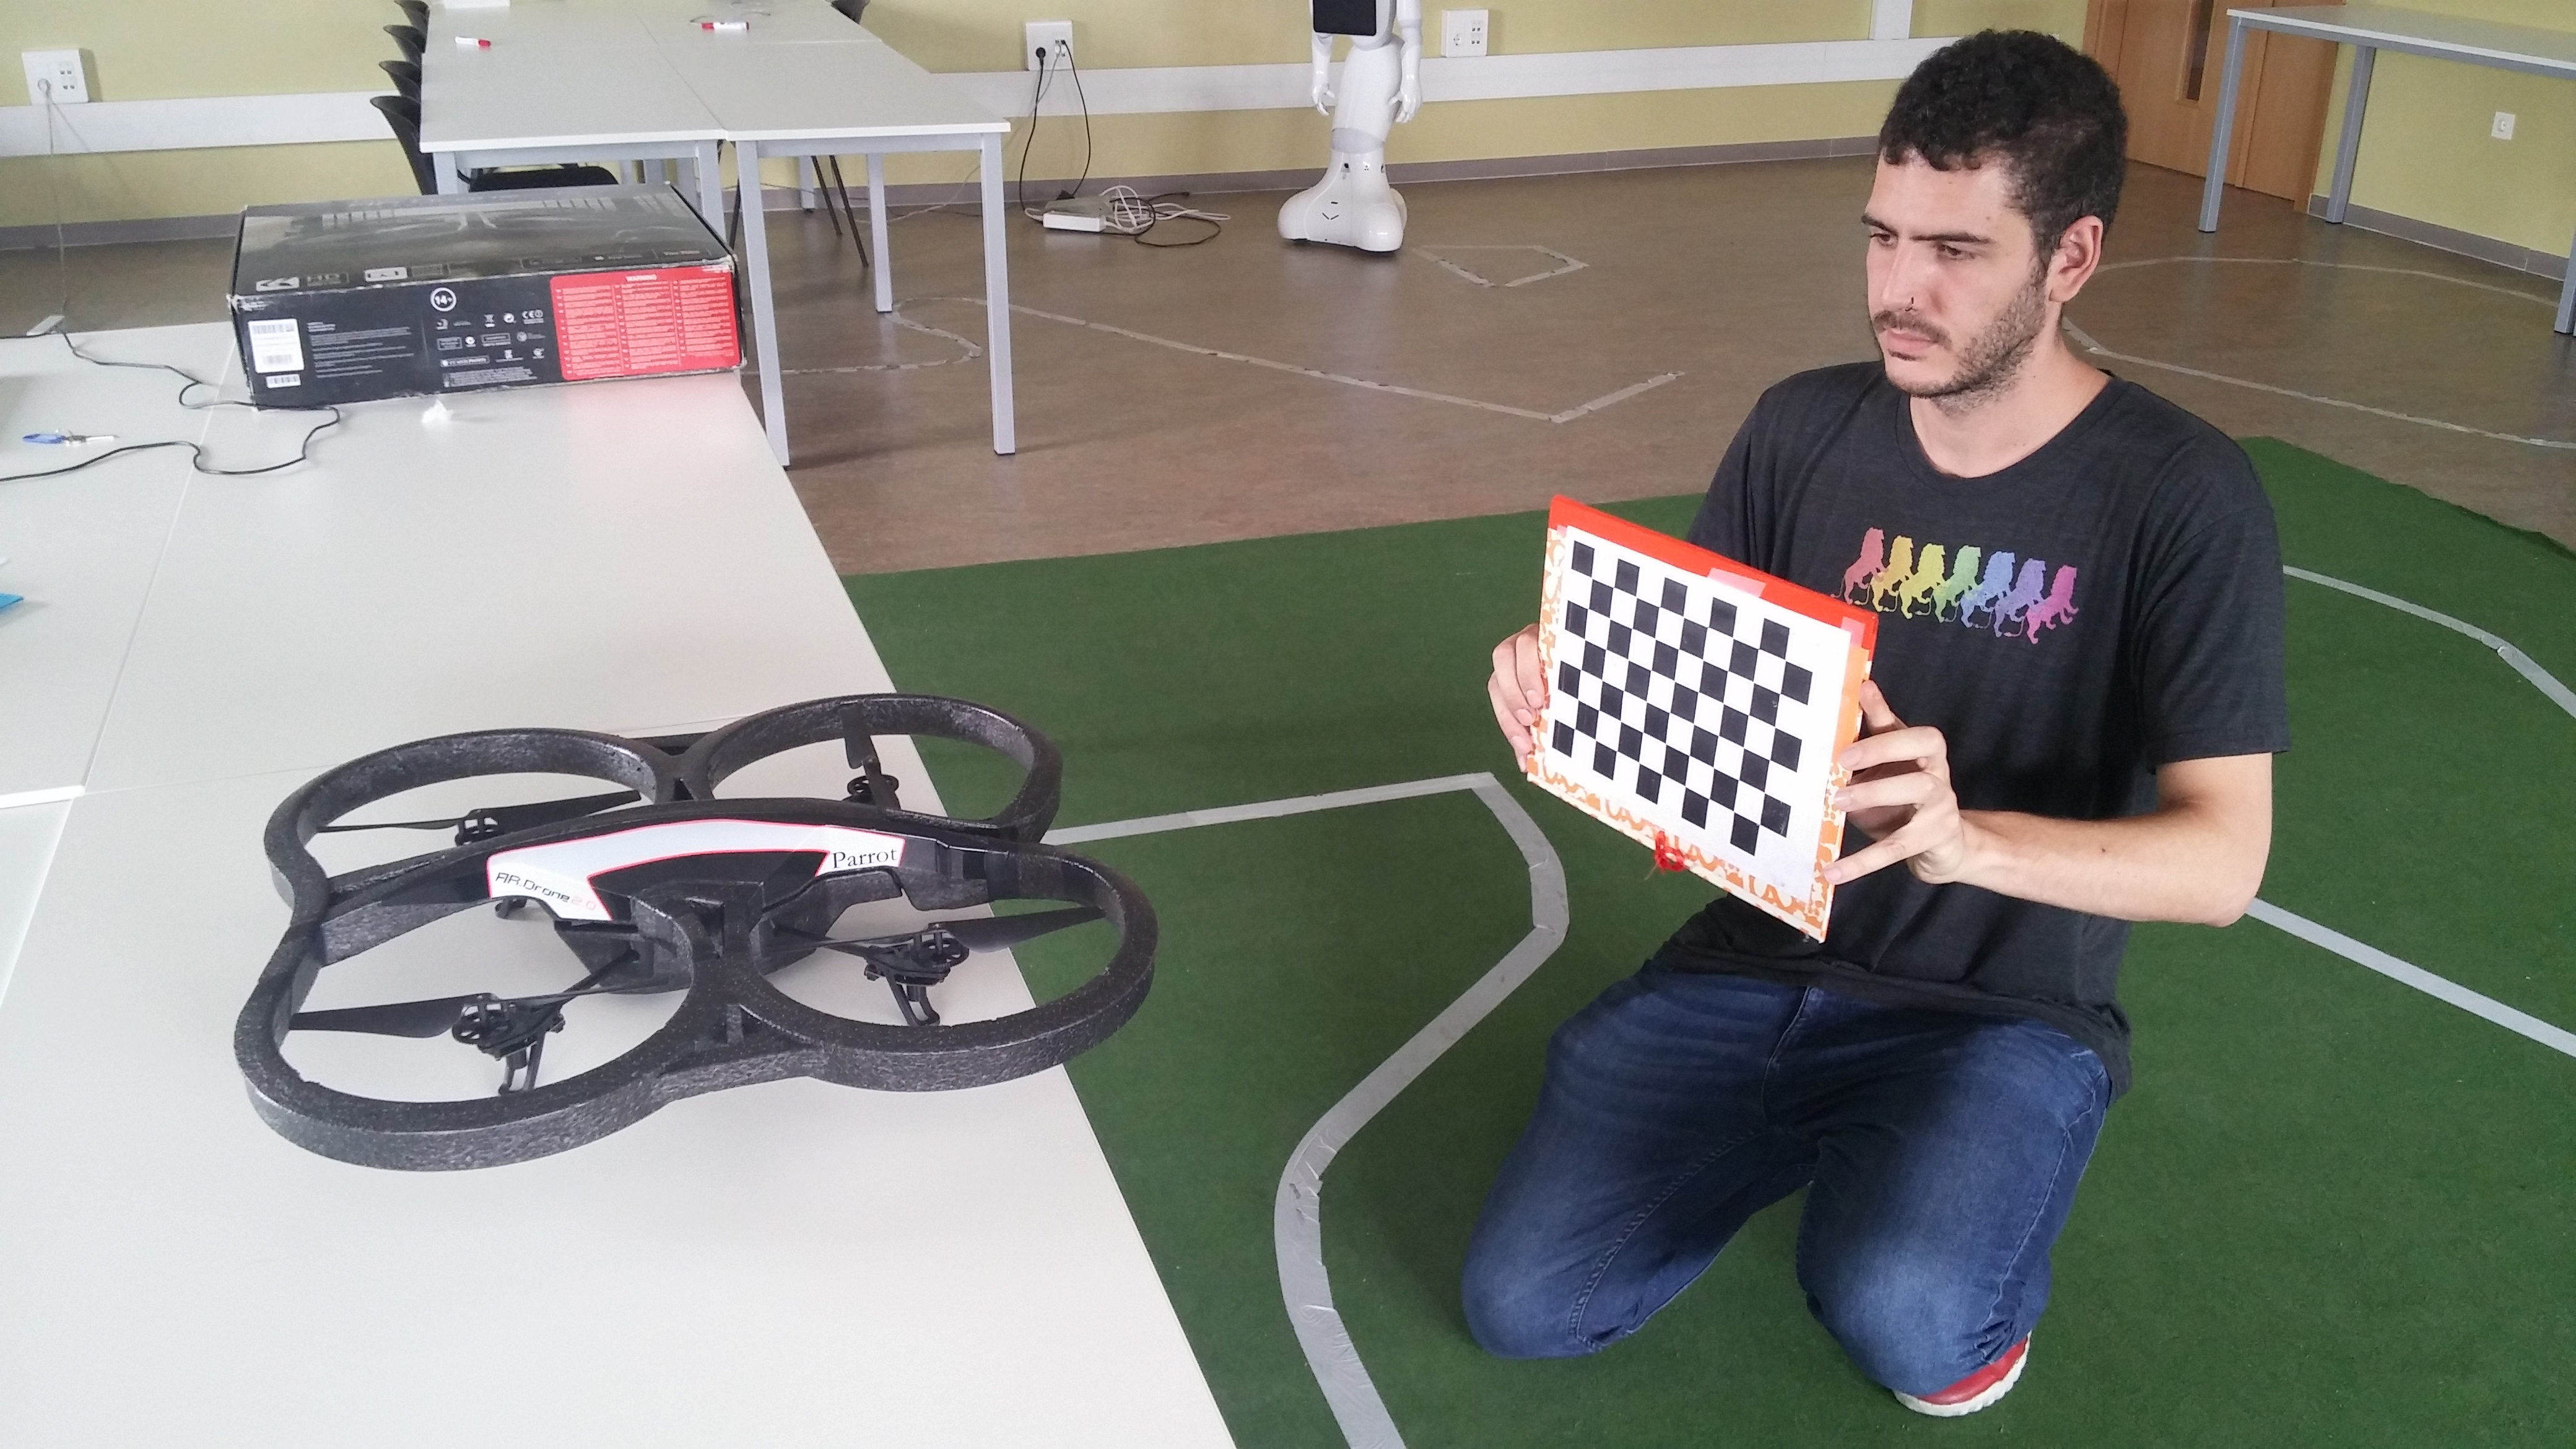
\includegraphics[width=6cm]{calibration.jpg}}
		\end{center}
		\caption{Real drone ArDrone2 and calibration of its onboard camera}
                \label{fig:calibration}
	\end{figure}
        
%        \subsubsection{Ardrone\_server}
	\textit{Ardrone\_server} is the JdeRobot driver that allows cammunication with the ArDrone quadrotor. It encloses the ArDrone SDK libraries provided by the manufacturer. There are six data interfaces offered by the driver, three of them for the sensor data, two for actuator commands and one for real-time configuration of the drone. The most important interfaces for this work are: \textit{CMDVel}, to send velocity commands; \textit{Ardrone\_extra}, that allows execution of complex maneuvers methods like taking off or landing; and \textit{Camera}, for onboard camera images.

%        \subsubsection{Uav\_viewer}
	\textit{Uav\_viewer} is a JdeRobot tool that allows the user to manually control an ArDrone through a Graphical User Interface (GUI). Drone sensor data are displayed on the GUI and two visual control pads for the control of the drone's movement are provided, including vertical and horizontal speed as well as angular speed along the Z axis. It can be connected both to real ArDrone as with a simulated quadrotor in Gazebo simulator.

%        \subsubsection{Quadrotor Gazebo plugin}
        JdeRobot includes one plugin for a quadrotor similar to \textit{ArDrone2.0} (Fig. \ref{fig:simnavigation}) in Gazebo simulator. It has been extensively used in this project, in particular on the initial stages. Gazebo is a multi-robot realistic simulator for both outdoor and indoor environments. It is able to simulate several robots with their sensors in a 3D world, and  
%This world can be created an personalized by the user, thanks to the tools provided for the integration with 3D models designed with SDF and the models included in Gazebo (\textit{TurtleBot} or \textit{Pioneer2}, from others). 
to emulate physical interactions between the objects in the 3D world thanks to its integration with physics libraries, such as \textit{Bullet} or \textit{Ogre}. The simulator is under constant development, and is maintained by the \textit{Open Source Robotics Foundation}. 

%Gazebo provides us with an extensive API, which is very well documented, to allow de users to develop their own plugins for their personalized robots and sensors.


\section{3D path following system}

%\subsection{Design}

The design of developed application is composed of two components as shown in Figure \ref{fig:design}. One of them is tasked with image analysis and 3D position estimation and the other one manages drone's movement and controls its position given the estimated location. Communication between both components is done through ICE interfaces.

% same with communication between the application and the cuadricopter.
%Each component has several modules running with threads that have different time cycles. One module of each component is serving as communications interface and manages shared memory, and the other ones correspond to graphic interface, information processing, algorithm application, etc.
	
	First, \textit{VisualLoc} component receives the images taken by the quadrotor's camera. It performs an analysis of the image looking for the presence of \textit{AprilTag} markers. Once the (several) markers are located, if any, it applies projective geometry to estimate the relative 3D position of the camera to each of the detected markers, and so, each 3D absolute camera position observation. In order to get an unique absolute 3D camera position it applies spatial fusion by a weighted average that filters observations. These weights take into account the 3D distance between the markers and the camera, giving higher weight to those marker detections closer to the camera. Finally, a temporal fusion is carried out by a \textit{Kalman Filter} to provide more robustness and the final estimation is sent to client components.

        Second, \textit{Navigator} component recieves the position estimations and generates a combination of velocities that control the movement of the quadcopter. It is a reactive controller. The position control is based on a predefined 3D path that the drone must follow. Given the prevalent horizontal feature of the indoor environments, the algorithm rests heavily on the rotation angle along the Z axis. The algorithm predicts the future position of the vehicle and adjusts the steering angle so the future position error in relation to the path is minimized.

        \begin{figure}[h]
          \begin{center}
            {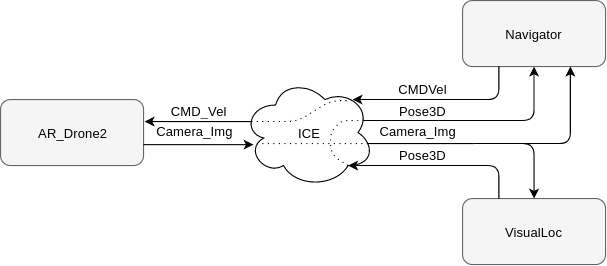
\includegraphics[width=\linewidth]{interactuacionproj.png}}
          \end{center}
          \caption{Global system design}
          \label{fig:design}
	\end{figure}
        
\subsection{Beacon based visual 3D localization}

%The self-localization task is carried out by the \textit{VisualLoc} component 

%Software implementation
	The software architecture of the \textit{VisualLoc} component consists of several modules. The \textit{MainWindow} module  interconnects the rest of the modules and implements a GUI. MainWindow also contains instances of the \textit{CameraManager} and \textit{World} classes. \textit{CameraManager} is in charge for the computer vision algorithms and \textit{World} renders a 3D world showing position estimation results. The \textit{Sensors} module manages ICE interfaces and shared memory between the rest of the modules. Following JdeRobot's standards, each of those modules is running on a different thread that periodically calls its \texttt{update()} method. Calling this method causes the modules to carry out their main tasks in an iterative way.
	
	A \textit{GeometryUtils} class has been developed in order to define a series of geometric calculus methods. Those methods include calculation of the intersection between planes and lines, generation of rotation matrices, or conversions between quaternions and euler angles. Pin-hole camera model has been used due to its simplicity and accuracy. The software structure that defines the camera is \textit{TPinHoleCamera} model, defined in \textit{progeo} library. %This structure is based on conical projections, meaning that all the light rays, at some point, pass through one unique point, the camera focus. 
In order to instance a \textit{TPinHoleCamera} object, camera parameters must be obtained by previous calibration of the real camera. Information regarding markers absolute position (map) and parameters of the onboard drone camera are loaded from two text files, \textit{markers.txt} and (\textit{camera.yml}.
	
	% \begin{figure}[h]
	% 	\begin{center}
	% 	{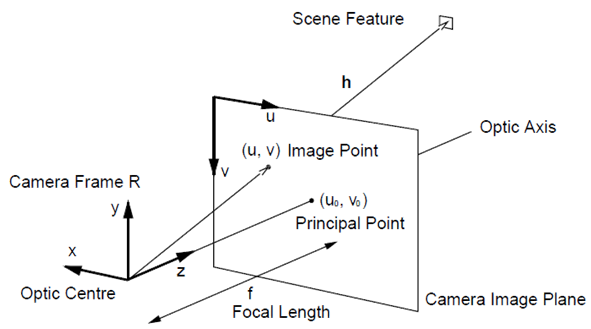
\includegraphics[width=\linewidth]{pinhole.png}}
	% 	\end{center}
	% 	\caption{Pin Hole Camera model}
	% \end{figure}
	
	
	The \textit{ProcessImage} method, contained in \textit{CameraManager}, processes the 2D image captured by the camera looking for markers, as well as estimates the 3D position of the camera. The markers found are instanced by \textit{MarkerInfo} class, which contains the information about each marker: id, size and position. Position is stored in two matrices, one with the position of the marker regarding the world and another one with the position of the world regarding the marker. The \textit{AprilTags} detection method is applied to a greyscale converted image, it generates an array containing all markers detected. The detected markers are highlighted on the original image and shown on the graphical user interface.
	
	Once the detection array is generated, each marker is located on the original image and a series of geometric operations are applied. Those operations start with the application of \textit{OpenCV}'s function \textit{SolvePnP}, which returns the relative position of the camera given a reference system composed of the correspondence between the 2D image points and the referred world's 3D points. Thus the translation and rotation vectors that determine the position of the marker in relation to the camera are obtained. In order to acquire the full RT matrix, \textit{OpenCV}'s function \textit{Rodrigues} is used. The matrix containing the position of the camera referred to the world is obtained by multiplying the calculated matrix and the matrix of the position of the marker in relation to the world.
	
	The position estimations for each marker are stored in an array, then, a \textit{spatial fusion} is applied by a weighted filter. This filter uses a different weight to each estimation based on the relative distance to the marker, closer markers get a higher weight. Particular weight values were set by experimental testing, analysing the distances where the system lost accuracy. The filter computes all the weights and then obtains a ratio for each estimation following equation (\ref{eq:ratio}). The final estimation is computed applying the weighted average of 3D coordinates of estimations, following the equation (\ref{eq:xyzfusion}). The rotation angles of the estimations are weighted following the special mechanism of equation (\ref{eq:alphafusion}), as they cannot be directly summed.
	
	\begin{equation}
	ratio_{i} = \frac{weight_{i}}{weight_{total}}
	\label{eq:ratio}
	\end{equation}
	
	\begin{equation}
	[x,y,z]_{fusion} = \sum_{i=1}^{n} ([x_{i},y_{i},z_{i}] \cdot ratio_{i})
	\label{eq:xyzfusion}
	\end{equation}
	
	\begin{equation}
	\alpha_{fusion} = \arctan \left( \frac{ \sum ( \sin \alpha_{i} \cdot ratio_{i} ) }{ \sum ( \cos \alpha_{i} \cdot ratio_{i} ) } \right)
	\label{eq:alphafusion}
	\end{equation}
	
	

        %% To accomplish that, a \textit{Kalman Filter} has been implemented. This filter was developed by Rudolf E. Kalman \cite{kalman:re} and its fuction is to estimate the state of a dynamic system using a series of measurements observerd over time, containing statistical noise. If it is a Gaussian noise, it works as an optimal estimator minimizing cuadratic error. \textit{Kalman Filter} estimate the state of a process $x$ in a given time $k$ (\ref{eq:xk}), provided the measure $z$ (\ref{eq:zk}). Where $w_{k}$ represents process noise and $v_{k}$ represents measure noise, asumming they are white gaussian noise and mutually independent.
	
	%% \begin{equation}
	%% x_{k} = A \cdot x_{k-1} + w_{k-1}
	%% \label{eq:xk}
	%% \end{equation}
	
	%% \begin{equation}
	%% z_{k} = H \cdot x_{k} + v_{k}
	%% \label{eq:zk}
	%% \end{equation}
	
	%% $A$ matrix relates the current state with the previous state, while $H$ matrix relates state and measure. Therefore, the algorithm estimates the current state of the process based on the previous state while getting feedback with noisy measures. The filter's equations can be divided in two groups, state prediction equations and measure update equations.
	
	%% The prediction equations (\ref{eq:xkk})(\ref{eq:Pk}) are shown below, where $\hat{x}_{k}^-$ is the state estimated a priori; $\hat{x}_{k-1}$ the state estimated a posterori; $P_{k}^-$ is the error covariance a priori; and $P_{k-1}$ the error covariance a posteriori.
	
	%% \begin{equation}
	%% \hat{x}_{k}^- = A \cdot \hat{x}_{k-1}
	%% \label{eq:xkk}
	%% \end{equation}
	
	%% \begin{equation}
	%% P_{k}^- = A \cdot P_{k-1} \cdot A^T + Q
	%% \label{eq:Pk}
	%% \end{equation}
	
	%% The measure update equations (\ref{eq:Kk})(\ref{eq:xkkk})(\ref{eq:Pkk}), that can be acknowledge as measure correction equations are shown below, where $(z_{k} - H \cdot \hat{x}_{k}^-)$ is the residue and $K_{k}$ is the Kalman gain that minimizes error a posterori.
	
	%% \begin{equation}
	%% K_{k} = \frac{P_{k}^- \cdot H^T}{H \cdot P_{k}^- \cdot H^T + R}
	%% \label{eq:Kk}
	%% \end{equation}

	%% \begin{equation}
	%% \hat{x}_{k} = \hat{x}_{k}^- + K_{k} \cdot (z_{k} - H \cdot \hat{x}_{k}^-)
	%% \label{eq:xkkk}
	%% \end{equation}

	%% \begin{equation}
	%% P_{k} = (I - K_{k} \cdot H) \cdot P_{k}^-
	%% \label{eq:Pkk}
	%% \end{equation}
	
        Due to occlusions or missing detections some markers may be not detected. Apart from the spatial fusion, a \textit{temporal fusion} is applied using a Kalman filter to provide more robust 3D position estimations on such conditions. With this method smoother results are obtained, while spike errors are also eliminated. The variation of a single pixel may result in a sudden change in the raw 3D position estimation, the \textit{Kalman Filter} mitigates the sudden variations that may occur. The values of the noise covariance matrices must be obtained with experimental testing in order to achieve desirable results. The final position estimation obtained through this filter is sent to \textit{Pilot} component. Additionally, in the GUI, the 3D world window shows the particular estimation for each marker and the filtered estimation.
	
\subsection{3D position control}

%	Position control is accomplished by the  \textit{Navigator} component. 

%software implementation
The \textit{Navigator} component consists of three modules: \textit{Interfaces}, \textit{Gui} and \textit{Pilot}. System inputs are ArDrone's camera images (\textit{Camera\_Img})); and position estimations given by \textit{VisualLoc} (\textit{Pose\_3D}). The outputs are a combination of linear and angular velocities (\textit{CMDVel}) and \textit{ArDrone\_extra} (for additional commands such as taking off or toggling cameras). Additionally, only in simulation, the absolute true position given by the simulator is available as input so the position estimation error can be calculated. The three modules provide an \texttt{update()} method that is called periodically by their corresponding thread asynchronically. 
%With this method, each of the modules run an iteration carrying out their main tasks.
	
	The \textit{Interfaces} module creates and manages the ICE communication interfaces. The needed parameters, such as IP address and port, are included in a text file that is loaded by ICE. It also manages shared memory between the rest of the modules, managing critical sections with a mutex. 

        The \textit{Gui} module implements a graphical user interface. \textit{PyQt} is the library used for the implementation. The interface shows (a) the images captured by the quadcopter's camera, (b) a real-time graph with the error between the vehicle's position and the desired path, and (c) a 3D world window rendered with \textit{OpenGL}. This world shows the quadcopter's position in relation to a coordinate axis and the path to follow, as well as the vehicle's trail. Additionally, a series of buttons are implemented allowing the user to manipulate the quadcopter with actions such as pausing or resuming movement, taking off, landing and toggling cameras.
	
	In the \textit{Pilot} module all the position information is processed and the velocity commands are generated. 
%Initially, a simple navigation system was developed which only relied on direction vectors from the vehicle to the corresponding path point. 
After some experimental testing, we reached to the conclusion that steering angle along Z axis (yaw) is a key factor for an accurate navigation, whereas lineal velocity can be constant while not making a big impact. In addition, the only linear velocities that matter are vertical velocity along Z axis and velocity along quadcopter's X axis. The velocity along quadcopter's Y axis is irrelevant. Thus, developing a control system around the steering angle was a suitable option.

 The algorithm is based on position prediction, so that steering angle adapts to the predicted error minimizing it. Only horizontal components are considered in the error prediction given the vertical components are minimal and don't affect steering control. It starts calculating the direction vector between the current position and the desired postion, that is, the corresponding path point following Eq.(\ref{eq:vecv}). Then unit vector is computed, Eq.(\ref{eq:uv}). In order to obtain the magnitude of the vertical and horizontal velocities while keeping linear velocity constant, unit vector must be decomposed. Vertical velocity is computed directly from the Z component of the unit vector and the predefined constant linear velocity $v_{k}$, Eq.(\ref{eq:vz}). Horizontal velocity is obtained by calculating the modulus of the X and Y component of the unit vector, Eq.(\ref{eq:vxy}).

	\begin{equation}
	\vec{V} = \vec{P_{ath}} - \vec{P_{ose}}
	\label{eq:vecv}
	\end{equation}
	
	\begin{equation}
	\vec{u}_{v} = \frac{\vec{V}}{|\vec{V}|}
	\label{eq:uv}
	\end{equation}
	
	\begin{equation}
	v_{x} = |\vec{u}_{vxy}| \cdot v_{k}
	\label{eq:vxy}
	\end{equation}
	
	\begin{equation}
	v_{z} = |\vec{u}_{vz}| \cdot v_{k}
	\label{eq:vz}
	\end{equation}
	
	Next step is obtaining the horizontal distance the vehicle will travel until the next controller iteration. That distance is calculated from the horizontal velocity previously obtained and the lapse of time between iterations, Eq.(\ref{eq:dtau}). In order to compute the future position regarding the current steering angle must be calculated. Considering that the received position rotation angles are expressed in quaternions, a transformation to euler angles must be done, Eq. (\ref{eq:euler}). Once those values are calculated, future position point is obtained following equations (\ref{eq:xf}) and (\ref{eq:yf}).
	
	\begin{equation}
	d_{\tau} = v_{x} \cdot \Delta_{t}
	\label{eq:dtau}
	\end{equation}

	\begin{equation}
	\theta_{z} = \arctan^2 \left( \frac{2 \cdot (q_{0} \cdot q_{3} +q_{1} \cdot q_{2})}{1-2 \cdot (q_{2}^2 + q_{3}^2)}\right)
	\label{eq:euler}
	\end{equation}		
	
	\begin{equation}
	X_{f} = d_{\tau} \cdot \cos \theta_{z} + x_{pose}
	\label{eq:xf}
	\end{equation}
	
	\begin{equation}
	Y_{f} = d_{\tau} \cdot \sin \theta_{z} + y_{pose}
	\label{eq:yf}
	\end{equation}
	
	In order to acquire the desired steering angle the future lateral error must be obtained. It has been computed from the difference between the predicted future position and the desired path point, Eq.(\ref{eq:le}). Finally, the steering angle is composed of the steering angle needed, $\delta{e}$, plus a steering angle gain that depends on the predicted future error, Eq.(\ref{eq:deltatheta}). The needed steering angle is obtained by calculating the yaw angle needed by the vehicle to face the navigation point. The factor $K_{g}$ is the gain rate of the steering adjustment and must be obtained experimentally. This adjustment ensures a minimization of the error by correcting vehicle's trajectory and smoothing its movement. The velocity commands sent to the quadricopter through the method \texttt{CMDVel()} are $v_{x}$, $v_{z}$ and $\delta_{\theta}$. 

	\begin{equation}
	L_{fe} = - \sin \theta_{z} \cdot ( X_{path} - X_{f} ) + \sin \theta_{z} \cdot ( Y_{path} - Y_{f} )
	\label{eq:le}
	\end{equation}

	\begin{equation}
	\delta_{\theta} = \sin \delta_{e} +  K_{g} \cdot ( L_{fe} / v_{x} )
	\label{eq:deltatheta}
	\end{equation}

\section{Experiments}

% experimentos con drone simulado
        Experimental tests have been performed on simulated and real drones. Simulations were run in \textit{Gazebo} simulator, creating a custom 3D world representing a typical flat where several AprilTags markers were placed (Figure \ref{fig:simnavigation}). The two system components were fine tunned separately on simulation. Then, once validated, the whole system was succesfully tested both on simulated and on a real scenarios.
        
	\begin{figure}[h!]
          \begin{center}
            {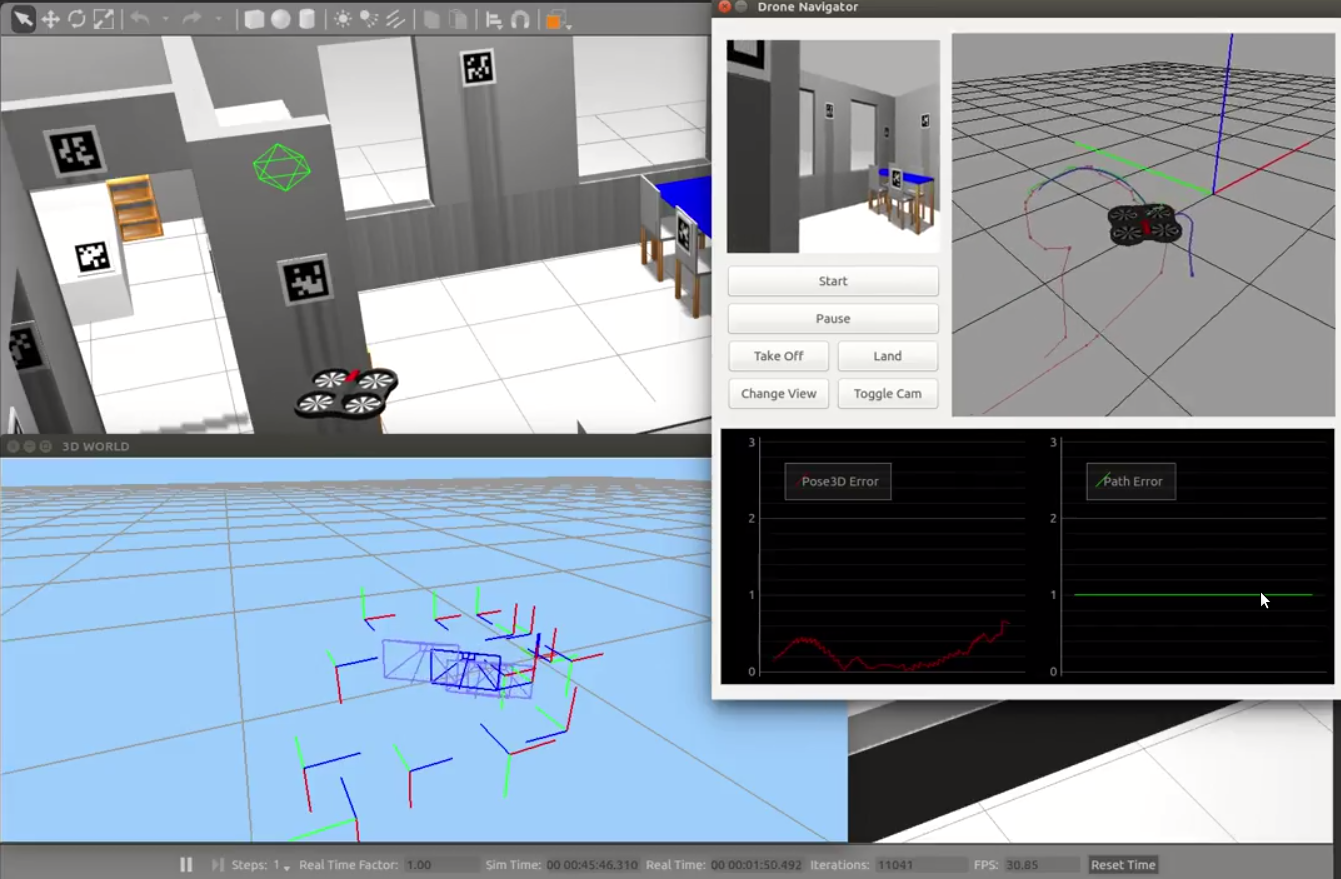
\includegraphics[width=12cm]{simnavigation.png}}
          \end{center}
          \label{fig:simnavigation}
          \caption{Position based control of a simulated drone}
	\end{figure}
        
% localization experiments
        Self-localization experiments in simulation showed high errors at the beginning. Through analysis, we detected that the algorithm was working properly but some used parameters were not correct. For instance, \textit{Kalman Filter} noise covariance matrices needed to be adjusted to properly model the real noise. In addition, used intrinsic parameters of the camera were not accurate and this caused localization errors. This was solved by a more accurate camera calibration. One of the most important conclusions of these experiments was that the markers needed to be bigger due to an erratic operation of the marker detection process caused by the high mobility of the aerial vehicle. The final marker size chosen was 25cm. Furthermore, it was noted that the accuracy of the position estimation algorithms decays rapidly when the distance of the camera to the marker is larger than 4 meters, confirming the results on \cite{lopezceron2016}.
	
% control experiments
	Control experiments in simulation showed good results from the beginning. We had to run several tests in order to find the proper parameters of the control algorithm. Vehicle's optimal speed is 0.1-0.4 m/s, and steering angle gain rate, $ K_{g}$ showed stable results within the range [0.1, 0.3]. The gain rate must be proportional to vehicle's speed in order to have a stable postion control. Lower gain rates are not enough to minimize the position error, while higher rates cause an erratic movement.
	
% experimentos con drone real
	The first real scenario experiments showed an unstable system behavior. Several tests were needed to find the correct parameters. Noise matrixes in the self-localization algorithm had to be re-adjusted so they could reflect the new noise model. Several marker sizes were also tested (17cm., 23cm.  and 33cm.), obtaining the best results with 33cm. markers. Also, quadcopter camera needed to be calibrated. The position control component also showed erratic behaviour due to the natural drift of the real vehicle and the magnitude of the velocity commands. Even though the drift caused by the slow movement of the vehicle could not be completeley corrected, speed parameters were adjusted so its impact was minimal. Furthermore, the movement of the vehicle caused a blurry effect on cameras, being angular speed a critical factor for this issue.
	
	\begin{figure}[h!]
          \begin{center}
            {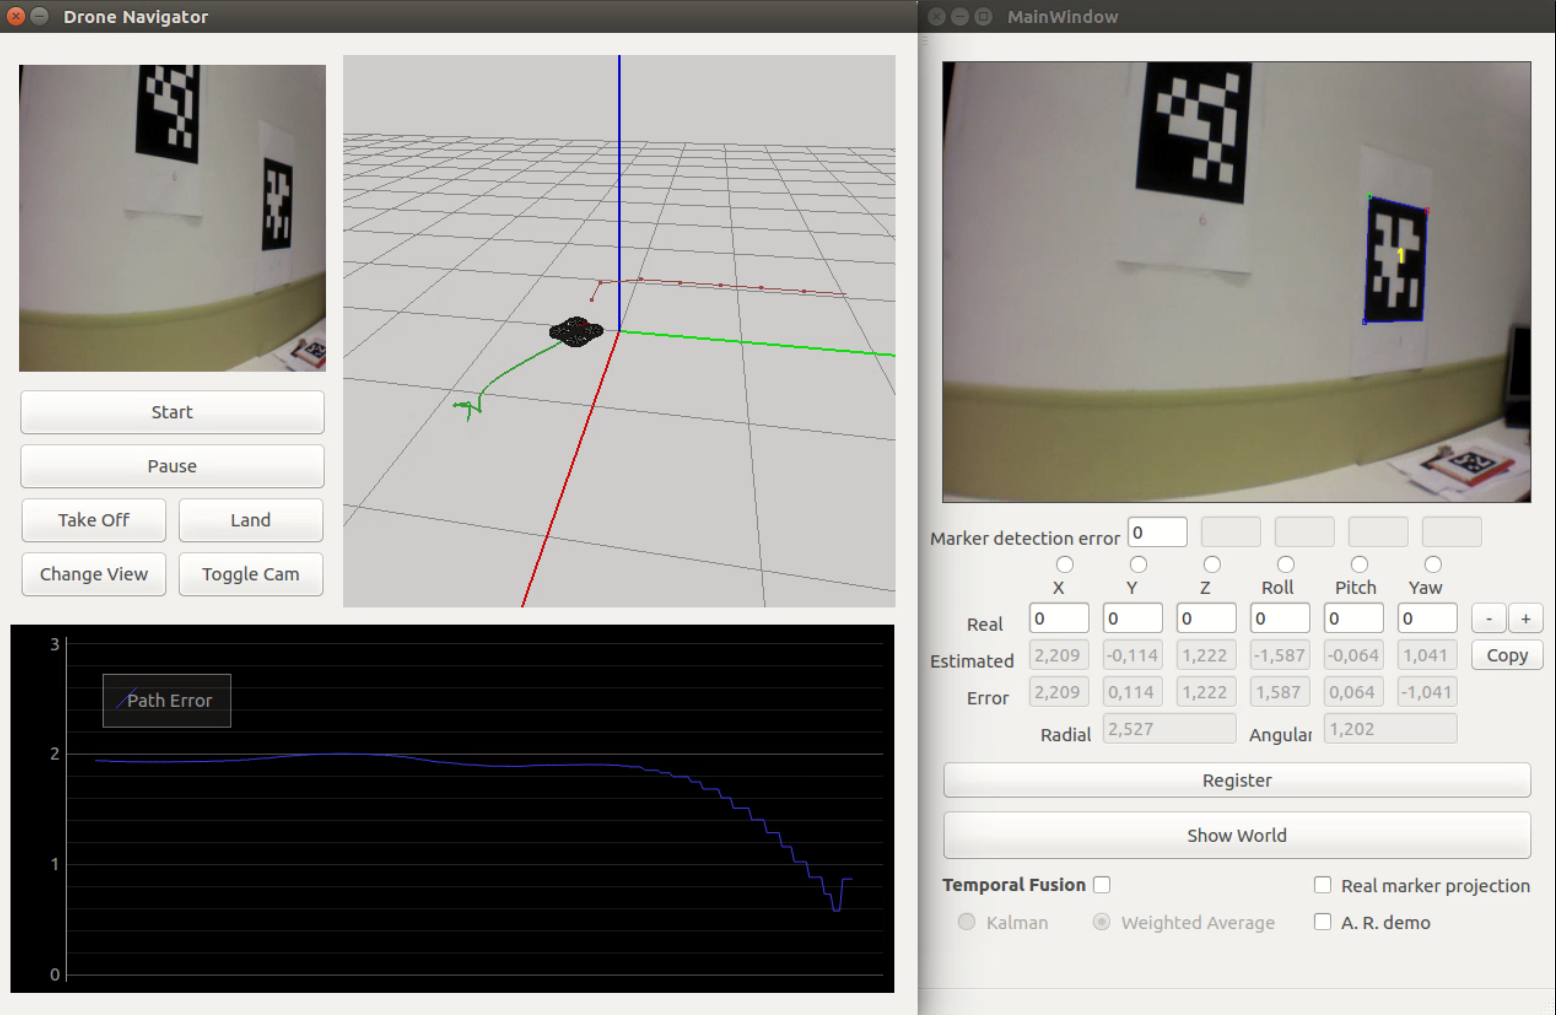
\includegraphics[width=12cm]{appcapture.png}}
          \end{center}
          \caption{Position based control of the real drone}
          \label{fig:realnavigation}
	\end{figure}
        

\section{Conclusions}

	We have designed and developed an autonomous quadcopter 3D path following system which is based on a visual markers self-localization technique on indoor scenarios. We have integrated several known technologies, adapting them to our purposes. The system has been succesfully validated on simulated and real quadcopters.

	Experimental results show that the system is limited in velocity due to the blurriness present in the images taken at high speed. Another key factor is the size of the markers. Taking into account such limitations and even though noisy data can affect the performance, it has proven to be stable and robust enough to follow simple 3D routes.

        Future lines involve the integration of other visual auto-localization algorithms without any markers at all. Furthermore, more exhaustive position control methods could be explored in order to cope with the quadcopter's drift.

        \section*{Acknowledgements}

        The research leading to these results has received funding from the RoboCity\-2030\--III\--CM project (Rob\'otica aplicada a la mejora de la calidad de vida de los ciudadanos. fase III; S2013/MIT-2748), funded by Programas de Actividades I+D en la Comunidad de Madrid and cofunded by Structural Funds of the EU. It has also received funding from
        %the RETOGAR project (TIN2016-76515-R) from the Spanish Ministerio de Econom\'{\i}a y Competitividad. 
%This research has been partially supported by the Spanish Government research funding ref.MINECO/FEDER TIN2015-69542-C2-1
the Banco de Santander and Universidad Rey Juan Carlos Funding Program for Excellence Research Groups (ref. Computer Vision and Image Processing (CVIP)).

%
% ---- Bibliography ----
%
\begin{thebibliography}{6}
\bibitem{wu2013}
Wu, A., Johnson, E.N., Kaess, M., Dellaert, F., Chowdhary, G.: Autonomous Flight in GPS-Denied Environments Using Monocular Vision and Inertial Sensors. J. Aerospace Inf. Sys.. 2013 Apr 1;10(4):172-86.

\bibitem{apvrille2013}
Apvrille, L., Dugelay, J.L., Ranft, B.: Indoor autonomous navigation of low-cost mavs using landmarks and 3d perception. Proc. Ocean and Coastal Observation, Sensors and Observing Systems. 2013 

\bibitem{forster2014}
Forster, C., Pizzoli, M., Scaramuzza, D.: SVO: Fast semi-direct monocular visual odometry, in Robotics and Automation (ICRA), 2014
IEEE International Conference on. IEEE, 2014, pp. 15–22.

\bibitem{engel2017}
J., Engel, Koltun, V., Cremers, D.,: Direct sparse odometry, IEEE Transactions on Pattern Analysis and Machine Intelligence, 2017

\bibitem{beul2015}
Beul, M., Krombach, N., Zhong, Y., Droeschel, D., Nieuwenhuisen, M., Behnke, S.: A High-performance MAV for Autonomous Navigation in Complex 3D Environments, International Conference on Unmanned Aircraft Systems (ICUAS) June 2015 \url{DOI: 10.1109/ICUAS.2015.7152417}

\bibitem{nikolic2014}
Nikolic, J., Leutenegger, S., Burri, M., Huerzeler, C., Rehder, J., Siegwart, R.: A UAV System for Inspection of Industrial Facilities, IEEE Aerospace Conference, 2013 \url{10.1109/AERO.2013.6496959}

\bibitem{lupashin2014}
Lupashin, S., Hehn, M., Mueller, M., Schoellig, A., Sherback, M., D’Andrea, R.: A platform for aerial robotics research and demonstration: The Flying Machine Arena, Mechatronics 24 (2014) 41–54

\bibitem{jimenez2014}
Jiménez, J., Zell, A.: Framework for Autonomous On-board Navigation with the AR.Drone, Journal of Intelligent \& Robotic Systems, January 2014, Volume 73, Issue 1–4, pp 401–412

\bibitem {dandrea2015}
Hehn, M., D'Andrea, R.: Real-Time Trajectory Generation for Quadrocopters, IEEE TRANSACTIONS ON ROBOTICS,  31(4), 2015

\bibitem {lopezceron2016}
López-Cerón, A., Cañas, J.M.: Accuracy analysis of marker-based 3D visual localization
 XXXVII Jornadas de Automática, Madrid, 2016 % \url{http://www.ncbi.nlm.nih.gov}

\bibitem{eolson}
Olson, E.: A robust and flexible visual fiducial system, IEEE International Conference on Robotics and Automation (ICRA), 3400-2407, 2011.

\bibitem{pestana2015}
  Pestana, J., Sanchez-Lopez, J.L., de la Puente, P., Carrio, A., Campoy, P.:
  A vision-based quadrotor multi-robot solution for the indoor autonomy challenge of the 2013 international micro air vehicle competition:
  Journal of Intelligent \& Robotic Systems, pages 1–20, 2015.
  
\bibitem{sanchezlopez2014}
  J.L. Sanchez-Lopez, J. Pestana, P. de la Puente, R. Suarez-Fernandez,and P. Campoy:
  A system for the design and development of vision-based multi-robot quadrotor swarms.
  In Unmanned Aircraft Systems (ICUAS), 2014 International Conference on, pages 640–648, May 2014
  
\bibitem{sanchezlopez2015}
  J. L. Sanchez-Lopez, J. Pestana, P. Puente, and P. Campoy:
  A reliable open-source system architecture for the fast designing and prototyping of autonomous multi-uav systems: Simulation and experimentation.
  Journal of Intelligent \& Robotic Systems, pages 1–19, 2015.

\bibitem{sanchezlopez2016}
  Jose Luis Sanchez-Lopez, Ramón A. Suárez Fernández, Hriday Bavle, Carlos Sampedro, Martin Molina, Jesus Pestana, and Pascual Campoy:
  AEROSTACK: An Architecture and Open-Source Software Framework for Aerial Robotics
  2016 International Conference on Unmanned Aircraft Systems (ICUAS) June 7-10, 2016. Arlington, VA USA

\bibitem{hernandez2014}
  Andres Hernandez, Harold Murcia, Cosmin Copot, Robin De Keyser:
  Model Predictive Path-Following Control of an AR.Drone Quadrotor 
  Memorias del XVI Congreso Latinoamericano de Control Automático, CLCA 2014, Octubre 14-17, 2014. Cancún, Quintana Roo, México

\bibitem{hernandez2013}
  Identification and Path Following Control of an AR.Drone Quadrotor
  Andres Hernandez, Cosmin Copot and Robin De Keyser Tudor Vlas and Ioan Nascu
  2013

\bibitem{rodriguezramos2016}
  Alejandro Rodriguez-Ramos, Carlos Sampedro, Adrian Carrio, Hriday Bavle, Ramon A. Suarez Fernandez, Zorana Milosevic, Pascual Campoy:  
  A Monocular Pose Estimation Strategy for UAV Autonomous Navigation in GNSS-denied Environments
  IMAV 2016
  
\bibitem{nguyen2014}
  Trung Nguyen, George K. I. Mann and Raymond G. Gosine
  Vision-Based Qualitative Path-Following Control of Quadrotor Aerial Vehicle
  2014 International Conference on Unmanned Aircraft Systems (ICUAS) May 27-30, 2014. Orlando, FL, USA

\bibitem{grabe2013}
  V. Grabe, M. Riedel, H.H. Bulthoff, P.R. Giordano, and A. Franchi:
  The telekyb framework for a modular and extendible ros-based quadrotor control. 
  In Mobile Robots (ECMR), 2013 European Conference on, pages 19–25, Sept 2013

\bibitem{kohlbrecher2014}
  Stefan Kohlbrecher, Johannes Meyer, Thorsten Graber, K Petersen, Oskar von Stryk, and U Klingauf. 
  Robocuprescue 2014-robot league team hector darmstadt (germany). 
  RoboCupRescue 2014, 2014.

\bibitem{michael2010}
  N. Michael, D. Mellinger, Q. Lindsey, and V. Kumar:
  The GRASP Multiple Micro-UAV Testbed, 
  IEEE Robotics Automation Magazine,vol. 17, pp. 56–65, September 2010.
\end{thebibliography}

        
\end{document}

